
\documentclass[10pt,journal,compsoc]{styles/IEEEtran}
\usepackage{styles/algorithm}
\usepackage[noend]{styles/algorithmic}
\usepackage{graphicx}
\usepackage{color}
\usepackage{listings}
\usepackage{amsmath}
\usepackage[utf8]{inputenc}
\usepackage[T1]{fontenc}

% *** CITATION PACKAGES ***
\ifCLASSOPTIONcompsoc
  % IEEE Computer Society needs nocompress option
  % requires cite.sty v4.0 or later (November 2003)
  \usepackage[noadjust]{cite}
\else
  % normal IEEE
  \usepackage{cite}
\fi

\title{Tarea 2: }

\author{Juan Gerardo Fuentes Almeida}

% The paper headers
\markboth{Tarea 2: Metodo de B\'usqueda en Linea}%
{Shell \MakeLowercase{\textit{et al.}}: Bare Advanced Demo of styles/IEEEtran.cls for Journals}

\IEEEtitleabstractindextext{%
\begin{abstract}
Se crea un programa que realiza una b\'usqueda en linea a partir de diferentes m\'etodos de c\'alculo de direcci\'on de descenso y tamaño de paso.
\end{abstract}
}

\begin{document}

% make the title area
\maketitle

\IEEEdisplaynontitleabstractindextext

\IEEEpeerreviewmaketitle

\section{Introducci\'on}

\IEEEPARstart{E}{n} esta pr\'actica se pretende encontrar el m\'inimo global de una funci\'on utilizando m\'etodos para calcular la direcci\'on de descenso $p_k$, tal como el Descenso del Gradiente y el m\'etodo de Newton; as\'i como la correcta estimaci\'on del tamaño de paso $\alpha_k$ que nos permita llegar al \'optimo en un tiempo m\'inimo. Se agregan tambi\'en los distintos criterios para la valoraci\'on de nuestra estimaci\'on de $\alpha_k$, tales como las condiciones de Wolfe y la condici\'on de Goldstein.\\


La funci\'on que minimizamos en esta pr\'actica es la funci\'on de Rosenbrock, en la cual el m\'inimo global se encuentra en un largo y plano valle de forma parab\'olica (Figura 1):
 
\begin{figure}[hbtp]
\centering
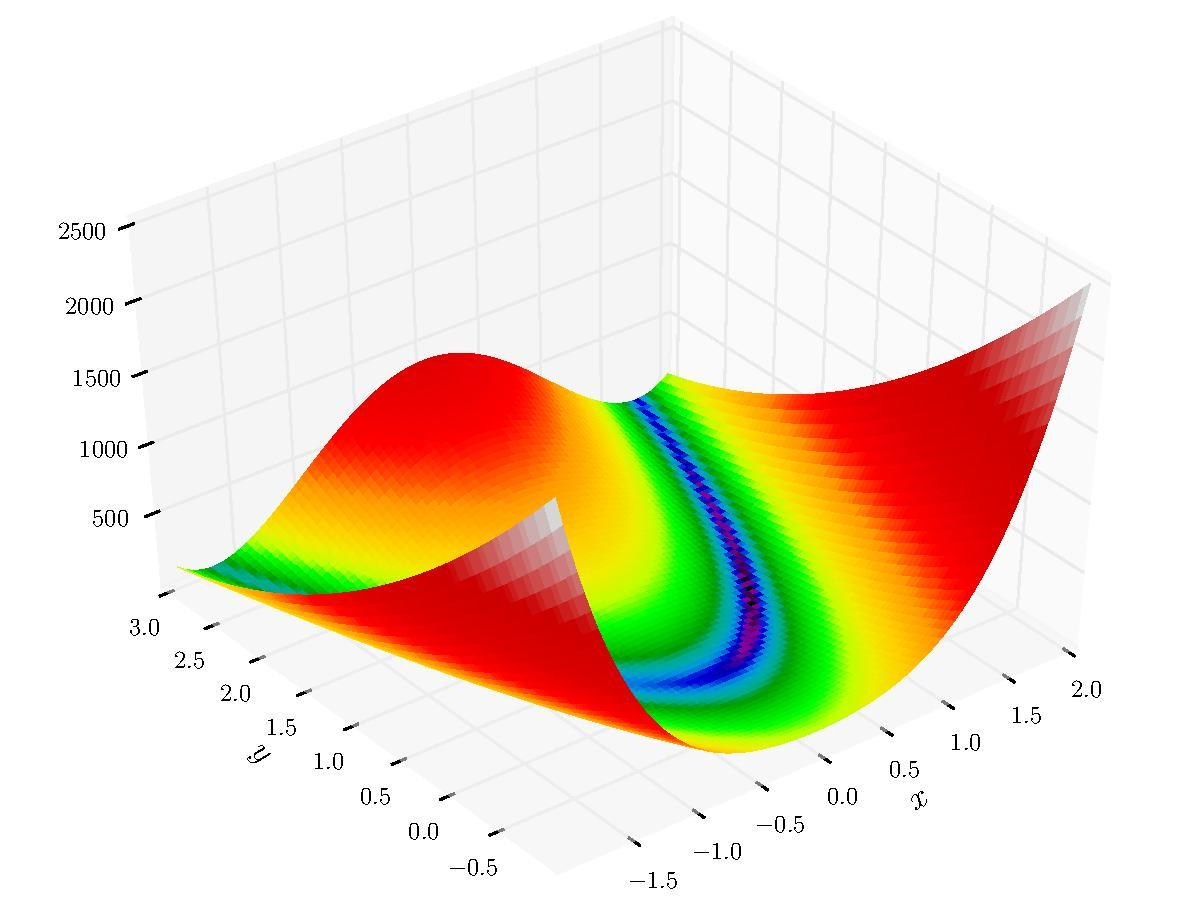
\includegraphics[width=0.4\textwidth]{rosenbrock.jpg}
\caption{Funcion Rosenbrock}
\end{figure}

Trataremos de encontrar el m\'inimo global de esta funci\'on en su forma 
bidimensional, el cual se conoce que se encuentra en (1,1) con $f(1,1)=0$:\\

$f(x_1,x_2)=100(x_2-x_1^2)^2+(1-x_1)^2$\\

el gradiente de esta funci\'on est\'a dado por

\[\nabla f(x_1,x_2)= \left( \begin{array}{cc}
-400x_1(x_2-x_1^2)-2(1-x_1) \\
200(x_2-x_1^2)\end{array} \right)\] 

\section{Teor\'ia}

\subsection{M\'etodo de Descenso de Gradiente}

Es un m\'etodo de optimizaci\'on de primer orden, en el cual se determina un m\'inimo local de una funci\'on tomando pasos proporcionales al negativo de su gradiente, y partiendo de que para una $\epsilon>0$ suficientemente peque\~na y una direccion de descenso $p_k$:\\

$f(x_k) + \epsilon\nabla f(x_k)^T p_k<f(x_k)$\\

Lo anterior implica que $\nabla f(x)^T p<0$. El algoritmo de Descenso del Gradiente consiste en tomar $p=-\nabla f(x)$ y recalcular las coordenadas del punto actual utilizando la expresi\'on general $x_{k+1}=x_k +\alpha_k p_k$. As\'i, en cada iteraci\'on nos acercamos al m\'inimo local de la funci\'on siguiendo la direcci\'on de descenso.


\subsection{Metodo de Newton}

En el m\'etodo de Newton, la direcci\'on de descenso se calcula a partir de la diferenciaci\'on de la aproximaci\'on de segundo orden de la serie de Taylor para calcular el m\'inimo:\\

$f(x+p_k)=f(x_k)+\nabla f(x_k)^T p_k + \frac{1}{2}p_k^{T}\nabla^{2} f(x_k)p_k$\\

$\Rightarrow \nabla f(x+p_k)=\nabla f(x_k)+\nabla^{2} f(x_k)p_k=0$\\

por tanto, la direcci\'on descenso esta dada por:\\

$p_k=-(\nabla^{2}f(x_k))^{-1} \nabla f(x_k)$\\

donde $\nabla^{2}f(x_k)$ denota el \emph{Hessiano} de la funci\'on $f(x_k)$

\[\nabla^{2}f(x_k)= \left( \begin{array}{cccc}
\frac{\partial^2 f}{\partial x_1^2} & \frac{\partial^2 f}{\partial x_1 \partial x_2} & \ldots & \frac{\partial^2 f}{\partial x_1 \partial x_n} \\
\frac{\partial^2 f}{\partial x_2 \partial x_1} & \frac{\partial^2 f}{\partial x_2^2} & \ldots & \frac{\partial^2 f}{\partial x_2 \partial x_n} \\
\vdots & \vdots & \ddots & \vdots \\
\frac{\partial^2 f}{\partial x_n \partial x_1} & \frac{\partial^2 f}{\partial x_n \partial x_2} & \ldots & \frac{\partial^2 f}{\partial x_n^2}
\end{array} \right)\] 

el cual es una matriz sim\'etrica que para este m\'etodo debe ser definida positiva.\\

\begin{figure}[hbtp]
\centering
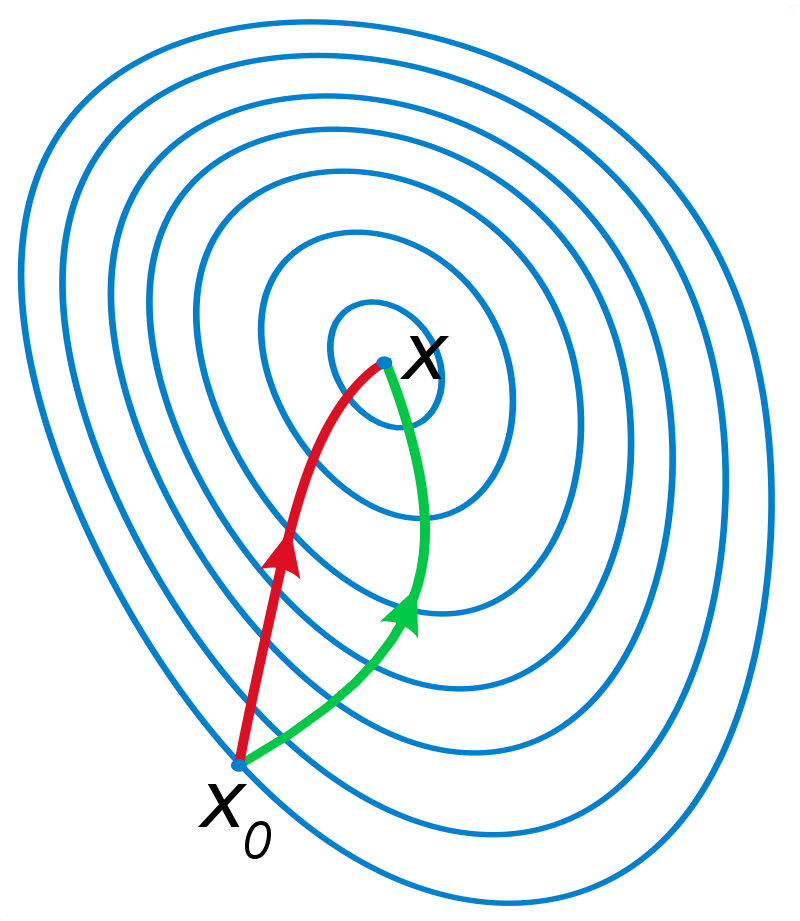
\includegraphics[width=0.3\textwidth]{newton.png}
\caption{Comparacion entre el metodo de Descenso del Gradiente (verde) y el metodo de Newton (rojo), el cual toma una ruta mas directa al minimo siguiendo la curvatura de la funcion}
\end{figure}

Computacionalmente, el inverso de esta matriz se obtiene aplicando la factorizaci\'on de Cholesky para el sistema de la forma $\textbf{Ax=b}$ en la expresi\'on:\\

$\nabla^{2}f(x_k) p_k=-\nabla f(x_k)$\\

y resolver el sistema de ecuaciones para $p_k$\\

La Figura 2 muestra una comparativa entre la direcci\'on que toman los vectores $p_k$ para cada m\'etodo, el m\'etodo de Newton en general llegar\'a al \'optimo local en menos iteraciones, ya que utiliza la informaci\'on del Hessiano para seguir la curvatura de la funci\'on mientras desciende.\\

\subsection{Condiciones de Wolfe}

\subsubsection{Suficiente descenso}

La condici\'on de suficiente descenso en la funci\'on objetivo para $\alpha_k$ esta dada por la siguiente desigualdad:\\

$f(x_k+\alpha p_k) \leq f(x_k)+c_1 \alpha \nabla f(x_k)^T p_k$\\

para alguna constante $c_1 \in (0,1)$. En otras palabras, la reduci\'on de $f$ debe ser proporcional tanto al tama\~no de paso $\alpha$ como a la derivada direccional $\nabla f(x_k)^T p_k$

\begin{figure}[hbtp]
\centering
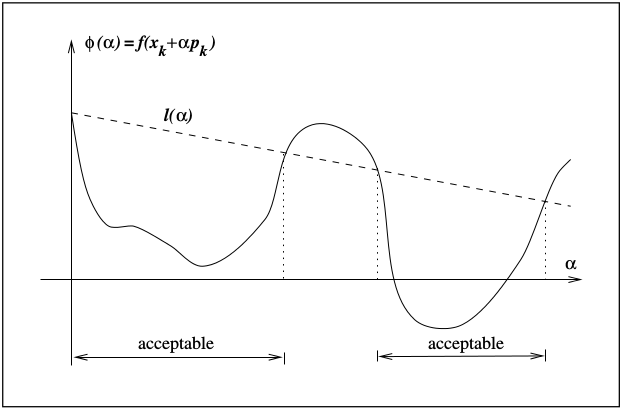
\includegraphics[width=0.45\textwidth]{sufdec.png}
\caption{Condici\'on de Suficiente Descenso. El lado derecho de la desigualdad se denota como $l(\alpha)$. }
\end{figure}

\subsubsection{Curvatura}

La condici\'on de suficiente descenso por s\'i sola no es suficiente para garantizar que el algoritmo haga un progreso razonable hacia el m\'inimo, porque como podemos ver en la Figura 3, esta condici\'on es satisfecha para valores suficientemente peque\~nos de $\alpha$. Para descartar pasos inaceptablemente peque\~nos se introduce un segundo requerimiento, denominado condici\'on de curvatura, el cual requiere que $\alpha$ satisfaga\\

$\nabla f(x_k+\alpha_k p_k)^Tp_k \geq c_2 \nabla f_k^T p_k$\\

para alguna constante $c_2 \in (c_1,1)$. Al ser el t\'ermino de la iquierda la derivada $\phi^{'} (\alpha_k)$, se garantiza que la pendiente  de $\phi$ no caiga por debajo de un l\'imite establecido por la constante $c_1$ y la direcci\'on de descenso.

\begin{figure}[hbtp]
\centering
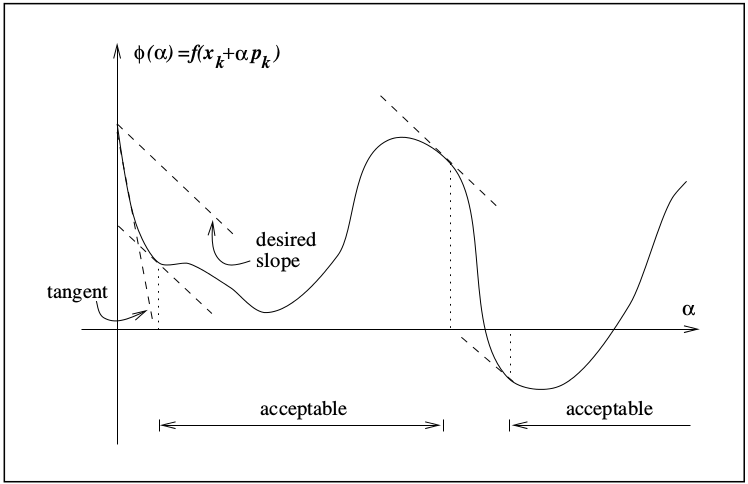
\includegraphics[width=0.45\textwidth]{curvature.png}
\caption{Condici\'on de curvatura }
\end{figure}

Las condiciones de suficiente descenso y de curvatura se conocen como condiciones d\'ebiles de Wolfe, mientras que las condiciones fuertes de Wolfe est\'an dadas por la condici\'on de suficiente descenso y una condici\'on determinada de la siguiente desigualdad:\\

 $|\nabla f(x_k+\alpha_k p_k)^Tp_k| \leq c_2| \nabla f_k^T p_k|$\\
 
Aqu\'i la diferencia radica en que ya no se permite que la derivada $\phi^{'}(\alpha_k)$ sea demasiado positiva, excluyendo puntos que se encuentran lejos de los puntos estacionarios de $\phi$.
 
 \subsection{Condiciones de Goldstein}
 
 Al igual que las condiciones de Wolfe, las condiciones de Goldstein garantizan que el tamano de paso $\alpha$ alcance suficiente descenso pero sin disminuir demasiado su magnitud:\\
 
 $f(x_k)+(1-c)\alpha\nabla f(x_k)^T p_k \leq f(x_k+\alpha p_k) \leq f(x_k)+c \alpha \nabla f(x_k)^T p_k$\\
 
 con $0<c<1/2$. La segunda desigualdad es la condici\'on de suficiente descenso, mientras que la primera desigualdad se introduce para controlar el tama\~no de paso (ver Figura 5).
 
\begin{figure}[hbtp]
\centering
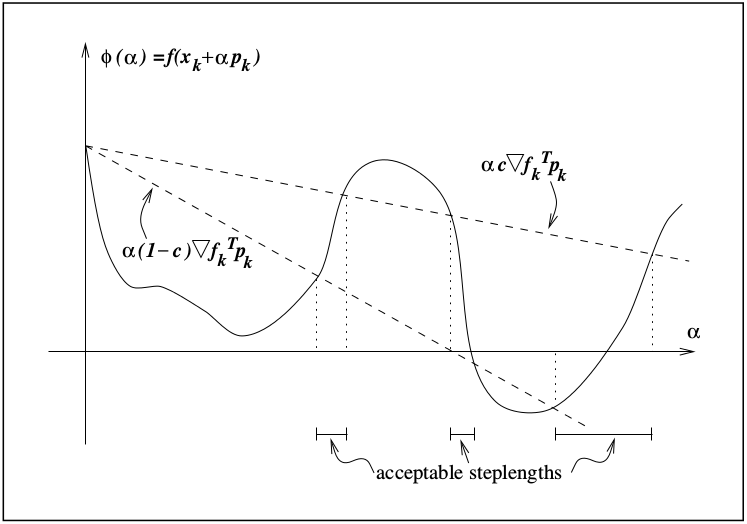
\includegraphics[width=0.45\textwidth]{goldstein.png}
\caption{Condiciones de Goldstein}
\end{figure}
 
\subsection{Estimaci\'on del tama\~no de paso}

\subsubsection{Modelos de Estimaci\'on}


Se obtienen a partir de la formulaci\'on de un modelo para $\phi_k(\alpha)=f(x_k+\alpha p_k)=f(x_{k+1})$.\\

Utilizamos el teorema de Taylor para ajustar la funci\'on a un modelo cuadr\'atico:

$m_k(\alpha)=f(x_k)+\alpha \nabla f(x_k)^T p_k + \frac{1}{2} \alpha^2 p_k^{T}\nabla^{2} f(x_k)p_k$\\

y se obtiene la siguiente estimaci\'on cuadr\'atica para $\alpha$:

$\alpha=\frac{\alpha_0^2 \phi'(0)}{2(\phi(0)+\alpha_0 \phi'(0)-\phi(\alpha_0))}$\\

con $\phi(0)=f_k$ y $\phi'(0)=\nabla f(x_k)^T p_k$. \\

Se puede proponer un modelo c\'ubico agregando el t\'ermino correspondiente al modelo ya establecido:\\

$m_3(\alpha)=a+b\alpha+c\alpha^2+d\alpha^3=\phi(\alpha)$\\

donde:\\
$m_3(0)=a \Rightarrow \phi(0)=a$\\
$m_3^{'}(0)=b \Rightarrow \phi'(0)=b$\\
$m_3^{"}(0)=2c \Rightarrow c=\frac{1}{2} \phi"(0)$\\

y para $d$:

$m_3(\alpha_0)=a+b\alpha_0+c\alpha_0^2+d\alpha_0^3=\phi(\alpha_0)$\\

$\Rightarrow d=\frac{1}{\alpha_0^3}[\phi(\alpha_0)-\phi(0)-\alpha_0 \phi0(0)-\frac{1}{2}\alpha_0^2 phi"(0)]$\\

y definimos $\alpha_3=arg min_{\alpha} m_3(\alpha) \Rightarrow \frac{\partial}{\partial \alpha}m_3(\alpha)=0$\\

$\Rightarrow b+c\alpha_3+3d\alpha_3^2=0$\\

Utilizando la formula general para calcular las raices de esta ecuaci\'on:\\

$\alpha_3=\frac{-c\pm \sqrt{c^2-3bd}}{3d}$

\subsubsection{Algoritmo de Backtracking con Inercia}

Otra forma de estimar $\alpha$ es con un algoritmo que dado un valor inicial, realice una actualizaci\'on hasta que alguna de las condiciones mencionadas anteriormente se cumpla. Por ejemplo, en el Algoritmo 1 se muestra el m\'etodo de Newton utilizando este m\'etodo de estimaci\'on.

 \begin{algorithm}   
	\caption{Backtracking con Inercia}  
	\label{alg1}
	\begin{algorithmic} 
		\REQUIRE Punto inicial $x$, $\alpha_0$ $maxIter$, $\epsilon$,$k \leftarrow 0$
		\WHILE{$k < maxIter$ \AND $error>\epsilon$}
		
			\STATE $G \leftarrow \nabla f_k$
			\STATE $H \leftarrow \nabla^{2}f(x_k)$
			\STATE $p_k \leftarrow -(\nabla^{2}f(x_k))^{-1} \nabla f(x_k)$
			\STATE $\alpha_k \leftarrow \alpha_2$ (modelo cuadratico)
			\STATE $tracking \leftarrow 0$,$count \leftarrow 0$,$maxcount$
			\WHILE{!Condition(Wolfe) \AND $count<maxcount$}
				\STATE $tracking \leftarrow tracking+1$
				\IF{$tracking>2$}
					\STATE $\alpha_k \leftarrow 3\alpha_k$
					\STATE $tracking \leftarrow 0$
				\ELSE
					\STATE $\alpha_k \leftarrow \alpha_k/2$				
				\ENDIF
				\STATE $count \leftarrow count+1$
			\ENDWHILE
			\STATE $x_{k+1} \leftarrow x_k+\alpha_k p_k$
			\STATE $error \leftarrow |x_{k+1}-x_k|$
			\STATE $x_{k+1} \leftarrow x_k$
			\STATE $k \leftarrow k+1$
		\ENDWHILE
		\RETURN $x$
	\end{algorithmic}
\end{algorithm}


\section{Resultados}

Como parte de la pr\'actica, se generaron 30 resultados para cada combinaci\'on de los m\'etodos descritos. A continuaci\'on se muestra una tabla comparativa entre cada m\'etodo; se documenta el n\'umero de iteraciones a las que convergi\'o el algoritmo, el tiempo de ejecuci\'on y la funci\'on evaluada en el punto m\'inimo obtenido. El algoritmo inicia con un valor aleatorio para $x_1$ y $x_2$ entre -5 y 15, y un $\alpha$ inicial est\'atico de 0.2:\\


\begin{tabular}{ |p{1.5cm}||p{0.7cm}|p{0.8cm}|p{1.5cm}|p{1.4cm}|p{0.6cm}|  }
 \hline
 \multicolumn{6}{|c|}{Metodo de Descenso de Gradiente} \\
 \hline
 Condicion&$\alpha$&Exitos&Iteraciones&Tiempo&$f_{min}$\\
 \hline
 Wolfe D & cuad & 25 & 16489 & 17.54042 & 0\\
 Wolfe D & cub & 29 & 5308 & 6.9045862 & 0\\
 Wolfe D & BT & 20 & 16773 & 111.0014 & 0\\
 Wolfe F & cuad & 24 & 13895 & 14.9569 & 0\\
 Wolfe F & cub & 30 & 5981 & 7.46247 & 0\\
 Wolfe F & BT & 21 & 18560 & 124.7305 & 0\\
 Goldstein & cuad & 22 & 1077 & 1.697818 & 0\\
 Goldstein & cub & 30 & 1889 & 2.108 & 0\\
 Goldstein & BT & 23 & 1064 & 1.2829 & 0\\
 \hline
\end{tabular}\\


La columna \emph{\'Exitos} indica cu\'antas de las 30 ejecuciones resultaron en el c\'alculo exitoso del m\'inimo, en los casos no exitosos se observ\'o que el algoritmo no pudo obtener el m\'inimo en el n\'umero de iteraciones m\'aximas dado ($1e6$), o que el valor de $\alpha$ se volv\'ia nulo y por consiguiente se originaba una falsa convergencia del algoritmo. El tiempo en ambas tablas esta dado en milisegundos.\\

\begin{tabular}{ |p{1.5cm}||p{0.7cm}|p{0.8cm}|p{1.5cm}|p{1.4cm}|p{0.6cm}|  }
 \hline
 \multicolumn{6}{|c|}{Metodo de Newton} \\
 \hline
 Condicion&$\alpha$&Exitos&Iteraciones&Tiempo&$f_{min}$\\
 \hline
 Wolfe D & cuad & 30 & 12 & 0.0157 & 0\\
 Wolfe D & cub & 30 & 38 & 0.0573 & 0\\
 Wolfe D & BT & 30 & 13 & 0.0613 & 0\\
 Wolfe F & cuad & 30 & 12 & 0.0159 & 0\\
 Wolfe F & cub & 30 & 38 & 0.0589 & 0\\
 Wolfe F & BT & 30 & 12 & 0.0612 & 0\\
 Goldstein & cuad & 30 & 133 & 0.1108 & 0\\
 Goldstein & cub & 30 & 138 & 0.1192 & 0\\
 Goldstein & BT & 30 & 151 & 0.1287 & 0\\
 \hline
\end{tabular}

\section{Conclusiones}

En general se observa que el m\'etodo de Descenso de Gradiente es mucho menos eficiente; aunque ya se ten\'ia previsto que el m\'etodo de Newton estaba formulado para llegar al punto m\'inimo mas r\'apido, no se hab\'ia estimado la magnitud de la diferencia en tiempos e iteraciones entre estos dos m\'etodos, tambi\'en se observa que no siempre el m\'etodo del Gradiente es capaz de llegar a un resultado, en cambio el m\'etodo de Newton siempre logra calcular el m\'inimo con exito.

En cuanto a la tabla que muestra el desempe\~no del m\'etodo de Newton, se observa que trabaja mejor con una de las condiciones de Wolfe, aunque bien la diferencia en n\'umero de iteraciones puede deberse a la elecci\'on de la constante $c$ para la condici\'on de Goldstein. Por otra parte, el m\'etodo funciona de manera excelente cuando se combina tambi\'en con el modelo cuadr\'atico para estimar $\alpha$, o bien con el algoritmo de backtracking con inercia, sin olvidar que en esta implementaci\'on en espec\'ifico esta combinado con el modelo cuadr\'atico.

\bibliographystyle{plain}
\bibliography{biblio}


\appendix
\section{Implementation details}
El programa est\'a implementado tomando en cuenta todas estandarizaciones indicadas en el curso.

Un \textit{makefile} ha sido generado, el cual soporta los comandos \textit{make}, \textit{run} and \textit{clean}. Para el tercer programa se incluye un script para correr las 30 ejecuciones de cada m\'etodo, los resultados se guardan en un archivo diferente para cada combinaci\'on, los argumentos del programa tienen el siguiente formato (todos son requeridos):\\

$arg1$ = 0(Descenso de Gradiente), 1(Newton)\\
$arg2$ = 0(Wolfe Debil), 1(Wolfe Fuerte), 2(Goldstein)\\
$arg3$ = 0(cuadratico), 1(cubico), 2(backtracking)\\


\end{document}


